\chapter{Results}\label{chap:results}

This chapter presents the results from applying the counterfactual analysis
methodology to a path-based knowledge graph recommender system. We start by examining
the initial recommendations generated by the recommender system for a random user.
Following this, we explore the outcomes of our counterfactual analysis
to understand how different attributes affect product recommendations.

\section{Case Study}
To provide a concrete example of our counterfactual analysis methodology process,
we will conduct a case study. This case study will
illustrate the application of our methodology, demonstrating its effectiveness and
potential insights.


\subsection{Initial Recommendations}
To initiate our analysis, we first examined the top 10 recommendations generated
by the CAFE recommender system engine for a specific user (user 0). These recommendations,
along with their associated paths and log probabilities, provide insight into the system's
decision-making process. Below, we present these recommendations and discuss their
implications.

\subsubsection*{Top 10 Recommendations for User 0:}
\begin{enumerate}
    \item \begin{center}
	{\footnotesize
	\begin{verbatim}
		 ([0, 261, 849],
		 [-4.5635014, -3.4569123],
		 ["mentions", "rev_described_by"])
	\end{verbatim}
	}
	\end{center}

    \item \begin{center}
	{\footnotesize
	\begin{verbatim}
		 ([0, 9826, 123],
		 [-5.4080114, -3.6974714],
		 ["mentions", "rev_described_by"])
	\end{verbatim}
	}
	\end{center}

    \item \begin{center}
	{\footnotesize
	\begin{verbatim}
		 ([0, 14974, 396],
		 [-5.5097566, -3.6836069],
		 ["mentions", "rev_described_by"])
	\end{verbatim}
	}
	\end{center}

    \item \begin{center}
	{\footnotesize
	\begin{verbatim}
		 ([0, 6797, 528],
		 [-5.648406, -3.7231576],
		 ["mentions", "rev_described_by"])
	\end{verbatim}
	}
	\end{center}

    \item \begin{center}
	{\footnotesize
	\begin{verbatim}
		 ([0, 856, 455, 330],
		 [-2.7392018, -1.455907, -3.5228138],
		 ["purchase", "also_viewed", "rev_also_bought"])
	\end{verbatim}
	}
	\end{center}

    \item \begin{center}
	{\footnotesize
	\begin{verbatim}
		 ([0, 856, 479, 626],
		 [-2.7392018, -2.2539396, -3.566442],
		 ["purchase", "also_viewed", "rev_also_bought"])
	\end{verbatim}
	}
	\end{center}

    \item \begin{center}
	{\footnotesize
	\begin{verbatim}
		 ([0, 856, 4350, 624],
		 [-2.7392018, -8.304826, -4.138239],
		 ["purchase", "described_by", "rev_described_by"])
	\end{verbatim}
	}
	\end{center}

    \item \begin{center}
	{\footnotesize
	\begin{verbatim}
		 ([0, 856, 13745, 241],
		 [-2.7392018, -8.540054, -4.213147],
		 ["purchase", "described_by", "rev_described_by"])
	\end{verbatim}
	}
	\end{center}

    \item \begin{center}
	{\footnotesize
	\begin{verbatim}
		 ([0, 856, 3327, 793],
		 [-2.7392018, -8.5651655, -4.2710376],
		 ["purchase", "described_by", "rev_described_by"])
	\end{verbatim}
	}
	\end{center}

    \item \begin{center}
	{\footnotesize
	\begin{verbatim}
		 ([0, 856, 3, 45],
		 [-2.7392018, -0.89929277, -3.0066423],
		 ["purchase", "produced_by", "rev_produced_by"])
	\end{verbatim}
	}
	\end{center}
\end{enumerate}

\subsubsection*{Analysis of Recommendations:}
Path Types: We observe four distinct path types in these recommendations:
\begin{itemize}
	\item 'mentions' $\rightarrow$ 'rev\_described\_by' (4 instances)

	\item 'purchase' $\rightarrow$ 'also\_viewed' $\rightarrow$ 'rev\_also\_bought'
		(2 instances)

	\item 'purchase' $\rightarrow$ 'described\_by' $\rightarrow$ 'rev\_described\_by'
		(3 instances)

	\item 'purchase' $\rightarrow$ 'produced\_by' $\rightarrow$ 'rev\_produced\_by'
		(1 instance)
\end{itemize}

\par
\vspace{1em}
The probability scores (represented as negative log-likelihoods)  [placeholder for logo probs definition] vary significantly
across the recommendations. Lower absolute values indicate higher
probabilities. 

In the following sections, we will explore how modifications to
these paths and attributes might alter the recommendation outcomes through our
counterfactual analysis.

\subsection{Counterfactual Analysis for User 0’s Recommendations}

% For user 0’s recommendations, we take the following path to perform the
% counterfactual analysis:
% \begin{center}
% 	[placeholder]
% \end{center}

Below is an example of a recommended path that user 0 is recommended product 45 based becuase of 
the brand of their previous purchases:
\begin{center}
	{\footnotesize
	\begin{verbatim}
		 ([0, 856, 3, 45],
		 [-2.7392018, -0.89929277, -3.0066423],
		 ["purchase", "produced_by", "rev_produced_by"])
	\end{verbatim}
	}
\end{center}
% show what the path represents
That with IDs converted to their corresponding real name for the attribute, it represents: 
\begin{align*}
	\text{user\_0} & \rightarrow \text{purchases}\rightarrow \text{product\_856}\rightarrow \text{produced\_by}\rightarrow \text{brand:Maybelline} \\
	               & \rightarrow \text{has\_produced}\rightarrow \text{product\_45}
\end{align*}

After removing the outlier nodes and determining the communities, as illustrated
in \fref{fig:attribute_selection}, we select the first-layer attributes that are connected to
a product that, in turn, is connected through the attributes of the recommended
product. This selection is made for all entities connected to the recommended product.
Based on these attibutes, counterfactual scenarios are constructed as described in the previous
section, and the recommender engine evaluates their plausability. 

% gephi of what happens
\begin{figure}[h!]
	\begin{center}
		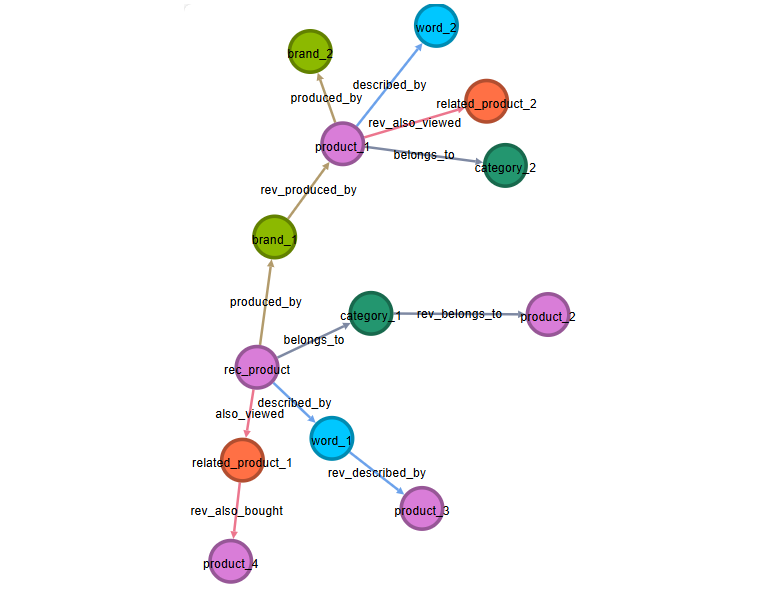
\includegraphics[width=0.9\columnwidth, keepaspectratio]{
			images/attribute_selection_4.png
		}
		\caption{Demonstration of First Layer Attribute Selection}
		\label{fig:attribute_selection}
	\end{center}
\end{figure}
\clearpage

% show what the lowest accepted score is
We consider the score of the path leading to the 10th recommended product as the
minimum acceptable threshold. If a counterfactual path achieves this score, it
indicates a scenario where the recommender engine assigns a score suggesting
that the user is likely to appreciate the recommendation.
% \clearpage


\fref{fig:cf_anaysis_example}
% gephi for all atttribute type paths
\begin{figure}[h!]
	\begin{center}
		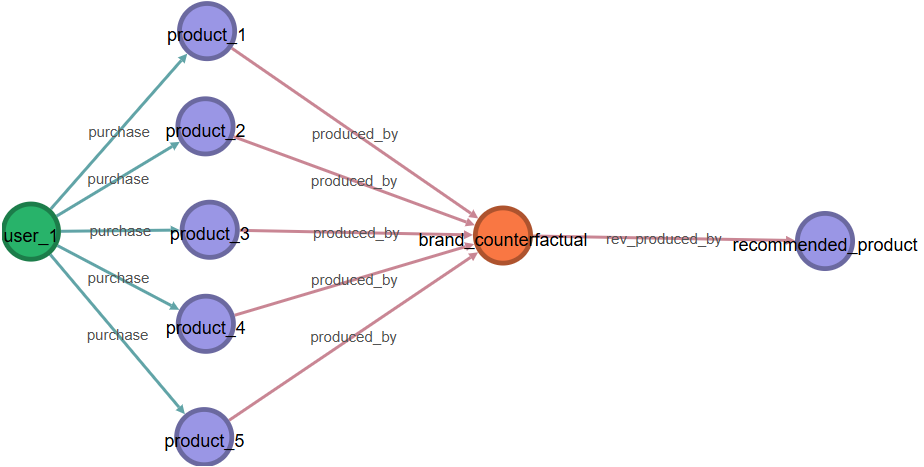
\includegraphics[width=0.9\columnwidth, keepaspectratio]{
			images/cf_anaysis_example.png
		}
		\caption{An Example of the Construction of Counterfactual Paths for an Attribute Evaluation}
		\label{fig:cf_anaysis_example}
	\end{center}
\end{figure}


% % gephi of what happens


The original attributes of the product in this recommendation are:\\
\noindent \textbf{Words} the product is described by:
\begin{multicols}{4}
	\raggedright marker\\ anybody\\ iti\\ bee\\ gosh\\ drawing\\ record\\ gloss\\ greatit\\
	rim\\ lightit\\ lipstick\\ liquid\\ wink\\ colorsensational\\ usage\\ downwards\\
	kinda\\ eh\\ z\\ berry\\ part\\ touch\\ satisfy\\ shine\\ mine\\ stiff\\ sun\\
	productmy\\ lipcolor\\ hubby\\ regular\\ turn\\ fabulous\\ full\\ precisely\\ morning\\
	point\\ mail\\ beyond\\ yes\\ ordered\\ remind\\ immediately\\ colorstay\\ pop\\
	ahead\\ sparkle\\ pleasedi\\ rosy\\ nude\\ folks\\ edge\\ insult\\ coloring\\
	itit\\ experienced\\ ohh\\ lipline\\ cherry\\ stung\\ senior\\ cracked\\
	indicative\\

	wine\\ stain\\ lid\\ arrive\\ person\\ tube\\ information\\ name\\ dayin\\ buff\\
	trash\\ least\\ lipstickthe\\ weird\\ waste\\ wonder\\ fricken\\ somewhat\\
	tint\\ delicious\\ colour\\ outside\\ ago\\ sorta\\ onto\\ rather\\ medicate\\
	fuscia\\ matte\\ taste\\ maybelline\\ assume\\ effect\\ loving\\ nature\\ palest\\
	cooltone\\ watery\\ slightly\\ tempt\\ hooked\\ mom\\ pigment\\ medium\\ gave\\
	total\\ dobut\\ layer\\ place\\ goodnot\\ bare\\ chemical\\ dissapointe\\ tacky\\
	reapp\\ sigh\\ itll\\ ugly\\ eos\\ periodical\\ cost\\ fact\\ luv\\ toilet\\

	mouth\\ application\\ complaint\\ waist\\ send\\ luck\\ exactly\\ else\\ kiss\\
	took\\ bother\\ placed\\ close\\ must\\ alot\\ m\\ wish\\ appear\\ stroke\\
	peel\\ drink\\ shipping\\ running\\ fix\\ delivery\\ intended\\ lasting\\ bag\\
	moist\\ fade\\ amaze\\ pieces\\ ready\\ hurt\\ recieve\\ productit\\ properly\\
	okay\\ bright\\ vibrant\\ raspberry\\ sting\\ uncomfortable\\ pen\\ eat\\
	koolaid\\ matter\\ overit\\ broken\\ orange\\ sell\\ scrub\\ means\\ certainly\\
	obviously\\ cake\\ putt\\ picture\\ eaten\\ reorder\\ tip\\ olay\\

	judge\\ manner\\ lipstain\\ doit\\ star\\ convenient\\ mys\\ inexpensive\\
	felttip\\ unfortunately\\ soon\\ understate\\ chapstick\\ low\\ future\\ gorgeous\\
	balm\\ damage\\ mention\\ applied\\ seller\\ inflexible\\ clump\\ bottleit\\
	roll\\ pick\\ yo\\ magic\\ practical\\ inevitable\\ making\\ true\\ defiant\\ sum\\
	n\\ reason\\ saturday\\ seal\\ confortable\\ poor\\ funky\\ fall\\ faith\\ pinkre\\
	worst\\ liner\\ guess\\ sharpie\\ cap\\ tend\\ darkish\\ working\\ open\\ thumb\\
	wild\\ napkin\\ paper\\ crayola\\ barely\\ fruit\\
\end{multicols}

\noindent \textbf{Brand} of the product is:

\begin{multicols}{4}
    \raggedright  % Ensures that the text is left-aligned and fits well in columns
	Maybelline
\end{multicols}

% \vspace{1em}  % Ensures 35pt vertical space after the text

\noindent \textbf{Categories} the product belongs to:
\begin{multicols}{4}
	\raggedright Makeup\\ Lips\\ Lip Stains\\ Beauty
\end{multicols}


\noindent \textbf{Related Products} that have been bought together, also bought, or also viewed with this product:
\begin{multicols}{4}
	\raggedright B006UEUJII\\ B004O3YCQ2\\ B00HF6S88I\\ B004Y9LAW0\\ B00HUAOE2S\\
	B00EYZR3E8\\ B00383O43U\\ B00IR6HW5A\\ B00HQLC91E\\ B0045KLPI2\\ B0051TSKTS\\
	B004EFHY0Q\\ B006UEUJV0\\ B00HWSNF00\\ B006UEUHXK\\ B00F9AALTG\\ B00303STIY\\
	B002YG5IZA\\ B00CTONUL6\\ B002YGB8D6\\ B00HF7I6ZM\\ B006HCJXBM\\ B0082D9R1K\\
	B00HWSNAPU\\ B00I4DRRXI\\ B00BEWRDUI\\ B00HWT32SE\\ B002YGBNSG\\ B00H3DAWO6\\
	B00A86SDLO\\ B006UET4XE\\ B002YGDCNU\\ B004ECH328\\ B004KOSZTK\\ B006UEUIJS\\
	B006UEUIUC\\ B00BSIPWS8\\ B006K5J3WA\\ B006UEUK82\\ B00AM3Z2XU\\ B00383KCCW\\
	B008GOR6O0\\ B00FORNVGO\\ B008JAPA7Q\\ B006UEUGWM\\ B00F0KHUDK\\ B005CYKJHI\\
	B0051TSLOW\\ B006UEUH80\\ B0082D9SUK\\ B004BCXAM8\\ B00CTOLDEC\\ B00HUAPZK8\\
	B004EF6DQC\\ B009FAPVJG\\ B004Y9LNEK\\ B004679FRM\\ B004O3YCLC\\ B001TK1I4M\\
	B004EFJW06\\ B0045KUO8E\\ B002YGB9JY\\ B004ECC24W\\ B004CKWWOQ\\ B00HUAO7ZM\\
	B006UEUI8E\\ B00HDE1672\\ B0057WJ1N8\\ B005CYK9HS\\ B007GMJ8Z8\\ B006UEUHLC\\
	B0051TSL10\\ B004EF8IGU\\ B00H2MSAVK\\ B00HDE0Q00\\ B005CYK6MG\\ B004O3ZPMW\\
	B00HWT1A8S\\ B008B2Z94Q\\ B004Y9JVWG\\ B004Y9LMN2\\ B0082D9RYM\\ B006UETDR6\\
	B004Y9LM8C\\ B00HU8W2BK\\ B002YGF4QS\\ B00F0KWBCU\\ B006XLA6U4\\ B009HVMVLY\\
	B00FZF3C46\\ B002YG6048\\ B00JULSPA2\\ B002YGF5FI\\ B00383Q11I\\ B002YGF5I0\\
	B005OGSO3K\\ B004ECGPMM\\ B006XM9M58\\ B005CYJKAU\\ B004ECIW3C\\ B0030GTYM6
\end{multicols}


\noindent And the plausible attributes approved by the recommender engine are as follows:
\noindent 
\textbf{BRAND}: If the product had one of these as \textbf{BRAND}, it would still be recommended
through that brand:
\begin{multicols}{4}
	\raggedright HEY\\ leegoal\\ e.l.f. Cosmetics\\ Coastal Scents\\ Mehron\\ Jordana\\
	Bonamart\\ MISSHA\\ Hard Candy\\ loel\\ Kevyn Aucoin\\ SHANY Cosmetics\\ Max
	Factor\\ NYX\\ Godefroy\\ Sleek\\ Essie\\ Kingmys\\ Physicians Formula\\ Epower
	Mall\\ Starry\\ COVERGIRL\\ L'Oreal Paris\\ Lime Crime\\ Sparkling Beauty\\ Benefit
	Cosmetics\\ Revlon\\ Neutrogena\\ Sigma Beauty\\ Crazy Cart\\ Ailunce\\ Maybelline\\
	divaderme\\ Cover Girl\\ Wonder Wedges
\end{multicols}


\textbf{Related Products}: If any of these \textbf{Related Products} were connected to the recommended product,
the product would still be recommended through that related product:
\begin{multicols}{4}
	\raggedright B001H270RQ\\ B004Y9GTYE\\ B00B1ZRTP2\\ B00EL1HZ34\\ B00BMW24TU\\
	B002UL5ZKC\\ B00HF6SJVY\\ B00B1DRA94\\ B008WG7X8Q\\ B003K16T06\\ B002ZTT9II\\
	B00HWSNF00\\ B002WTC38O\\ B009K7X26I\\ B009HVMVLY\\ B005BF1M10\\ B002ULRAQE\\
	B004Y9M81W\\ B006UET4XE\\ B000CECSAO\\ B008FX7B9M\\ B000US0804\\ B001KYQA1S\\
	B006UEUI8E\\ B0030GTYM6\\ B002ISV7B8\\ B001HKR6WM\\ B004Y9LAW0\\ B004X1QY20\\
	B0013TM9UQ\\ B004BCX8B6\\ B001KYNZM0\\ B00303STIY\\ B00112BUBO\\ B00150LT40\\
	B004B3YC9M\\ B005OZH88I\\ B002UL10M4\\ B009ZB6MKM\\ B006OZEYR0\\ B004BCXAM8\\
	B004Y9LM8C\\ B0048KSGZO\\ B00DHQCJTO\\ B004M7WKKK\\ B0013L3XMM\\ B00FAEOCP0\\
	B001IB0NOS\\ B006UETDGC\\ B00KVBZAXK\\ B008GOR6O0\\ B004Y9GV60\\ B00FORNVGO\\
	B005UKZAJG\\ B003FKSVMG\\ B009WI3RZQ\\ B005EIIEQA\\ B006OZF3DY\\ B004Y9GVZG
\end{multicols}


\textbf{WORDS}: No word was verified, as if it was connected to the recommended product,
the product would be recommended through that word.



% Plausable \textbf{Words} verified by the counterfactual analysis:
% \begin{center}
% 	[placeholder]
% \end{center}


% \noindent Plausable \textbf{Brands} verified by the counterfactual analysis:
% \noindent Plausable \textbf{Categories} verified by the counterfactual analysis:
% \noindent Plausable \textbf{Related Products} verified by the counterfactual analysis:

The plausible scenarios work in favor of the explainability by demonstrating how
changes in specific product attributes, such as the brand or ingredients, could
still lead to a strong recommendation for the user. This enhances the system's transparency
by showing that the recommendation is not solely dependent on a single brand or fixed
set of attributes but can adapt to user preferences, as long as the core
characteristics of the product align with the user's needs.

\subsection*{Counterfactual Analysis Results and Their Interpretation}
For a given path to undergo counterfactual analysis, the counterfactual
scenarios derived from validated neighbors are evaluated by the recommender
system engine. The plausible attributes, according to the engine, are presented in
four groups: brand, category, word, and related products. The revelations of
each group of attributes are as follows:

\begin{itemize}[leftmargin=1cm] % Adjust left margin as needed
	\item \textbf{Brand Influence:} If the recommended product had been associated
		with a different brand within the same category and still met the threshold
		score, this implies that brand substitutability exists within certain user preferences,
		indicating flexibility in brand choice.

	\item \textbf{Word Influence from Reviews:} Altering descriptive attributes (for
		example adding “animal cruelty free”, “organic”) and finding that the product
		still surpasses the score threshold suggests the potential descriptive qualities
		that the user will find favorable for the recommended product.

	\item \textbf{Connectivity and Exposure:} Introducing hypothetical connections
		to recommended product and products (e.g., often bought together or viewed together)
		and observing their impact on the recommendation score could highlight
		potential for cross-selling strategies.
\end{itemize}

\subsection{Key Marketing Findings and Enhancing Marketing Strategies}

This section outlines the marketing insights derived from our counterfactual analysis:
\begin{enumerate}
	\item \textbf{Brand Associations:} The wide range of brands identified in the
		counterfactual analysis suggests that the recommended product has broad
		appeal across different market segments.

	\item \textbf{Key Descriptors:} Words like "stays" and "eyelash" provide
		insights into the product's key selling points, which could be emphasized in
		marketing materials.

	\item \textbf{Related Product Opportunities:} The identification of related
		products that influence recommendations presents cross-selling and bundling
		opportunities.
\end{enumerate}

These insights can be utilized to enhance marketing strategies in several ways:
\begin{enumerate}
	\item \textbf{Targeted Advertising:} By understanding the diverse attributes
		that lead to a recommendation, marketers can create more targeted and effective
		advertising campaigns.

	\item \textbf{Product Positioning:} The variety of associated categories and
		brands allows for flexible product positioning to appeal to different
		customer segments.

	\item \textbf{Content Marketing:} The identified key words and categories can
		inform content creation, ensuring that product descriptions and marketing materials
		align with the attributes that drive recommendations.

	\item \textbf{Cross-Promotion:} The related products identified in the
		analysis can guide cross-promotion strategies, potentially increasing sales across
		product lines.

	\item \textbf{Dynamic Pricing:} Understanding the range of brands associated
		with a product can inform pricing strategies, potentially allowing for price
		adjustments based on perceived brand value.

	\item \textbf{Product Development:} Insights into the attributes that drive
		recommendations can inform future product development, ensuring new products
		are designed with recommendation potential in mind.
\end{enumerate}

By using these marketing insights derived from our counterfactual analysis,
businesses can improve their recommendation systems and enhance their overall
marketing effectiveness.

\section{Ablation Study: Impact of Community Detection and Outlier Removal}

In addition to the qualitative case study presented in Section 4.1, a further
evaluation was conducted to assess the impact of the proposed filtering approach
on counterfactual generation. Specifically, we performed an ablation study to
compare runs with and without the key filtering steps—community detection and
outlier removal. This section details the ablation settings and provides quantitative
evidence that these filtering methods significantly reduce the search space while
preserving most of the useful counterfactual scenarios.

\subsection{Experimental Setup}
The objective of the ablation study was to measure how community detection (CD) and
outlier removal (OR) affect:

\begin{itemize}
	\item The number of candidate attributes (words, brands, categories, related products)
		considered in counterfactual analysis,

	\item The number of final “eligible” counterfactuals that pass the scoring threshold
		(i.e., would remain recommended in plausible “what-if” scenarios), and

	\item The overall number of scenarios tested (which reflects computational
		complexity).
\end{itemize}

We considered four distinct configurations:

\begin{enumerate}
	\item \textbf{Filtering = OFF:} No community detection and no outlier removal.

	\item \textbf{Filtering = ON:} Both community detection and outlier removal
		enabled.

	\item \textbf{Community\_Filter = ON, Outlier\_Filter = OFF:} Only community
		detection is applied.

	\item \textbf{Community\_Filter = OFF, Outlier\_Filter = ON:} Only outlier
		removal is applied.
\end{enumerate}

For each configuration, the system generated counterfactual scenarios for the
same set of user–product pairs. We measured:

\begin{itemize}
	\item The count of “related” attributes detected for each type (categories, brands,
		words, related products),

	\item Their proportion relative to the total knowledge graph (e.g.,
		$\text{categories\_percentage}= \frac{\text{retained categories}}{\text{total
		possible categories}}$),

	\item The total number of counterfactual scenarios enumerated ($\text{num\_cf\_scenarios}$),
		and

	\item The number of “eligible” (plausible) scenarios that exceed the scoring threshold
		($\text{num\_eligible\_scenarios}$).
\end{itemize}

\subsection{Results Overview}
Table \ref{tab:ablation_user0} summarizes the ablation results for the first
user discussed in Section 4.1, while Tables \ref{tab:ablation_user1}–\ref{tab:ablation_user4}
present corresponding results for the four additional users.


\begin{table}[htbp]
    \centering
    \caption{Ablation Study Results for User 0 (Community vs. Outlier Filtering).}
    \label{tab:ablation_user0}
    \begin{tabular}{lcccc}
        \hline
        Configuration    & Categories & Words  & Related Products & Counterfactuals \\
        \hline
        Filtering OFF    & 15,361     & 25,532 & 1,470,000       & 23              \\
        Filtering ON     & 7,500      & 12,000 & 382,000         & 21              \\
        Community ON, Outlier OFF & \dots & \dots & \dots & \dots \\
        Community OFF, Outlier ON & \dots & \dots & \dots & \dots \\
        \hline
    \end{tabular}
\end{table}


\subsection{Comparison Across Additional Users}

To validate the consistency of these findings, we repeated the same four
configurations for four other users. Tables \ref{tab:ablation_user1}–\ref{tab:ablation_user4}
show comparable results:


\begin{table}[htbp]
    \centering
    \caption{Results for User 1}
    \label{tab:ablation_user1}
    \resizebox{\textwidth}{!}{
    \begin{tabular}{lcccc}
        \hline
        Configuration & Categories & Words & Related Products & Counterfactuals \\
        \hline
        ...           & ...        & ...   & ...              & ...             \\
        \hline
    \end{tabular}
    }
\end{table}

\begin{table}[htbp]
    \centering
    \caption{Results for User 2}
    \label{tab:ablation_user2}
    \resizebox{\textwidth}{!}{
    \begin{tabular}{lcccc}
        \hline
        Configuration & Categories & Words & Related Products & Counterfactuals \\
        \hline
        ...           & ...        & ...   & ...              & ...             \\
        \hline
    \end{tabular}
    }
\end{table}

\FloatBarrier

\begin{table}[htbp]
    \centering
    \caption{Results for User 3}
    \label{tab:ablation_user3}
    \resizebox{\textwidth}{!}{
    \begin{tabular}{lcccc}
        \hline
        Configuration & Categories & Words & Related Products & Counterfactuals \\
        \hline
        ...           & ...        & ...   & ...              & ...             \\
        \hline
    \end{tabular}
    }
\end{table}

\FloatBarrier

\begin{table}[htbp]
    \centering
    \caption{Results for User 4}
    \label{tab:ablation_user4}
    \resizebox{\textwidth}{!}{
    \begin{tabular}{lcccc}
        \hline
        Configuration & Categories & Words & Related Products & Counterfactuals \\
        \hline
        ...           & ...        & ...   & ...              & ...             \\
        \hline
    \end{tabular}
    }
\end{table}


\subsection{Discussion}

These ablation results suggest that community detection and outlier removal both
play a crucial role in making counterfactual analysis more tractable while
preserving the high-value explanations. By pruning commonly connected but uninformative
nodes (outlier removal) and confining search to semantically relevant subgraphs (community
detection), the method avoids exploring an exponential number of low-impact
“what-if” scenarios. As shown in the tables, filtering often cuts the scenario
space by over 70\%, yet retains 90\% or more of the ultimately eligible counterfactuals.

Such substantial computational savings is essential in practical deployments where
real-time or near-real-time responsiveness is needed. Furthermore, the minimal impact
on the final results indicates that the pruned attributes are largely redundant or
uninformative from a user-modeling standpoint. This not only streamlines the
analysis but also improves interpretability by limiting the number of potential
counterfactual explanations that analysts or end-users must review.



\section{Limitations and Challenges}

\begin{enumerate}
	\item \textbf{Computational Complexity:} The process of generating and
		evaluating counterfactual scenarios for each recommendation is
		computationally intensive, especially for large-scale knowledge graphs. This
		limits the real-time application of this method in production recommender
		systems.

	\item \textbf{Attribute Independence Assumption:} Our analysis treats each
		attribute independently, which may not always reflect real-world scenarios where
		attributes can be correlated. This simplification might lead to some
		unrealistic counterfactual scenarios.

	\item \textbf{Threshold Sensitivity:} The choice of threshold score for
		determining relevant counterfactuals can significantly impact the results. Finding
		the optimal threshold that balances inclusivity and relevance remains a challenge.

	\item \textbf{Temporal Aspects:} Our analysis doesn't account for temporal
		changes in user preferences or product popularity, which could affect the relevance
		of counterfactual scenarios over time.

	\item \textbf{Bias Reinforcement:} There's a risk that focusing on attributes
		that lead to recommendations could reinforce existing biases in the
		recommender system.
\end{enumerate}